\documentclass[aspectratio=169]{../latex_main/tntbeamer}  % you can pass all options of the beamer class, e.g., 'handout' or 'aspectratio=43'
\usepackage{dsfont}
\usepackage{bm}
\usepackage[english]{babel}
\usepackage[T1]{fontenc}
%\usepackage[utf8]{inputenc}
\usepackage{graphicx}
\graphicspath{ {./figures/} }
\usepackage{algorithm}
\usepackage[ruled,vlined,algo2e,linesnumbered]{algorithm2e}
\usepackage{hyperref}
\usepackage{booktabs}
\usepackage{mathtools}

\usepackage{amsmath,amssymb}

\DeclareMathOperator*{\argmax}{arg\,max}
\DeclareMathOperator*{\argmin}{arg\,min}

\usepackage{pgfplots}
\pgfplotsset{compat=1.16}
\usepackage{tikz}
\usetikzlibrary{trees} 
\usetikzlibrary{shapes.geometric}
\usetikzlibrary{positioning,shapes,shadows,arrows,calc,mindmap}
\usetikzlibrary{positioning,fadings,through}
\usetikzlibrary{decorations.pathreplacing}
\usetikzlibrary{intersections}
\pgfdeclarelayer{background}
\pgfdeclarelayer{foreground}
\pgfsetlayers{background,main,foreground}
\tikzstyle{activity}=[rectangle, draw=black, rounded corners, text centered, text width=8em]
\tikzstyle{data}=[rectangle, draw=black, text centered, text width=8em]
\tikzstyle{myarrow}=[->, thick, draw=black]

% Define the layers to draw the diagram
\pgfdeclarelayer{background}
\pgfdeclarelayer{foreground}
\pgfsetlayers{background,main,foreground}

% Requires XeLaTeX or LuaLaTeX
\usepackage{unicode-math}

\usepackage{fontspec}
%\setsansfont{Arial}
\setsansfont{RotisSansSerifStd}[ 
Path=../latex_main/fonts/,
Extension = .otf,
UprightFont = *-Regular,  % or *-Light
BoldFont = *-ExtraBold,  % or *-Bold
ItalicFont = *-Italic
]
\setmonofont{Cascadia Mono}[
Scale=0.8
]

% scale factor adapted; mathrm font added (Benjamin Spitschan @TNT, 2021-06-01)
%\setmathfont[Scale=1.05]{Libertinus Math}
%\setmathrm[Scale=1.05]{Libertinus Math}

% other available math fonts are (not exhaustive)
% Latin Modern Math
% XITS Math
% Libertinus Math
% Asana Math
% Fira Math
% TeX Gyre Pagella Math
% TeX Gyre Bonum Math
% TeX Gyre Schola Math
% TeX Gyre Termes Math

% Literature References
\newcommand{\lit}[2]{\href{#2}{\footnotesize\color{black!60}[#1]}}

%%% Beamer Customization
%----------------------------------------------------------------------
% (Don't) Show sections in frame header. Options: 'sections', 'sections light', empty
\setbeamertemplate{headline}{empty}

% Add header logo for normal frames
\setheaderimage{
	% 
\includegraphics[height=\logoheight]{figures/TNT_darkv4.pdf}
	
\includegraphics[height=\logoheight]{../latex_main/figures/luh_logo_rgb_0_80_155.pdf}
	% 
\includegraphics[height=\logoheight]{figures/logo_tntluh.pdf}
}

% Header logo for title page
\settitleheaderimage{
	% 
\includegraphics[height=\logoheight]{figures/TNT_darkv4.pdf}
	
\includegraphics[height=\logoheight]{../latex_main/figures/luh_logo_rgb_0_80_155.pdf}
	% 
\includegraphics[height=\logoheight]{figures/logo_tntluh.pdf}
}

% Title page: tntdefault 
\setbeamertemplate{title page}[tntdefault]  % or luhstyle
% Add optional title image here
%\addtitlepageimagedefault{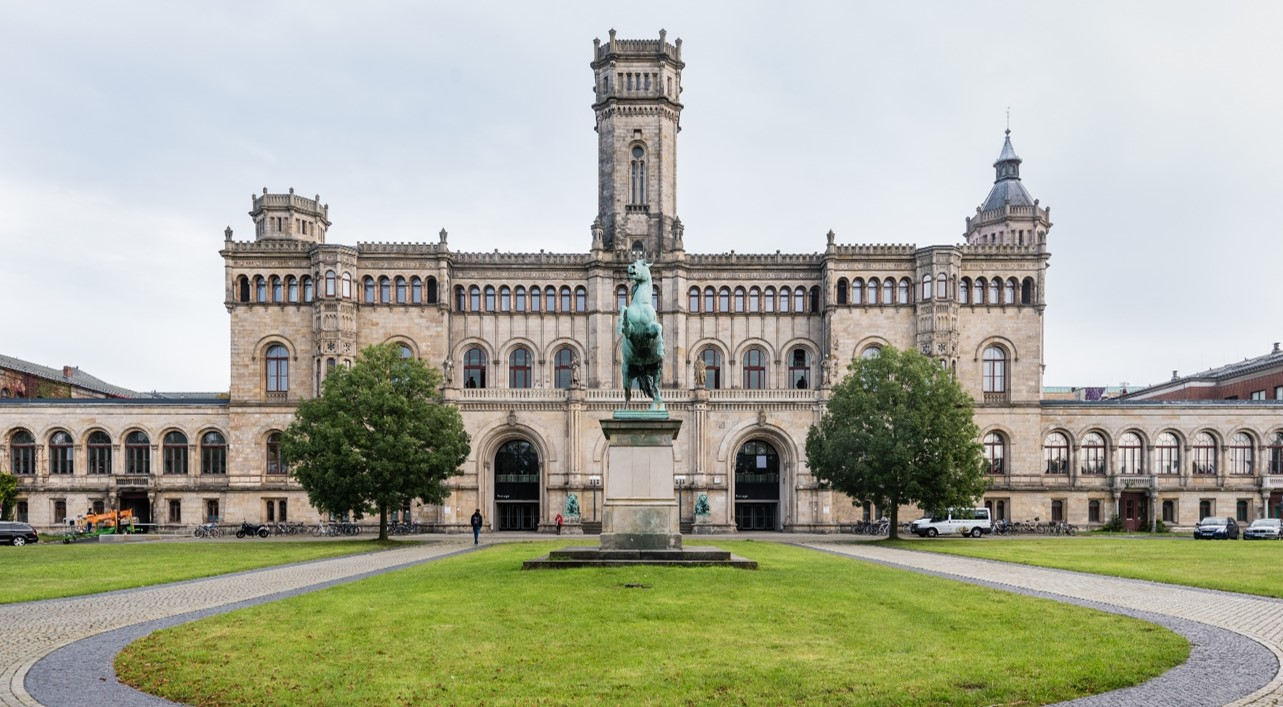
\includegraphics[width=0.65\textwidth]{figures/luh_default_presentation_title_image.jpg}}

% Title page: luhstyle
% \setbeamertemplate{title page}[luhstyle]
% % Add optional title image here
% \addtitlepageimage{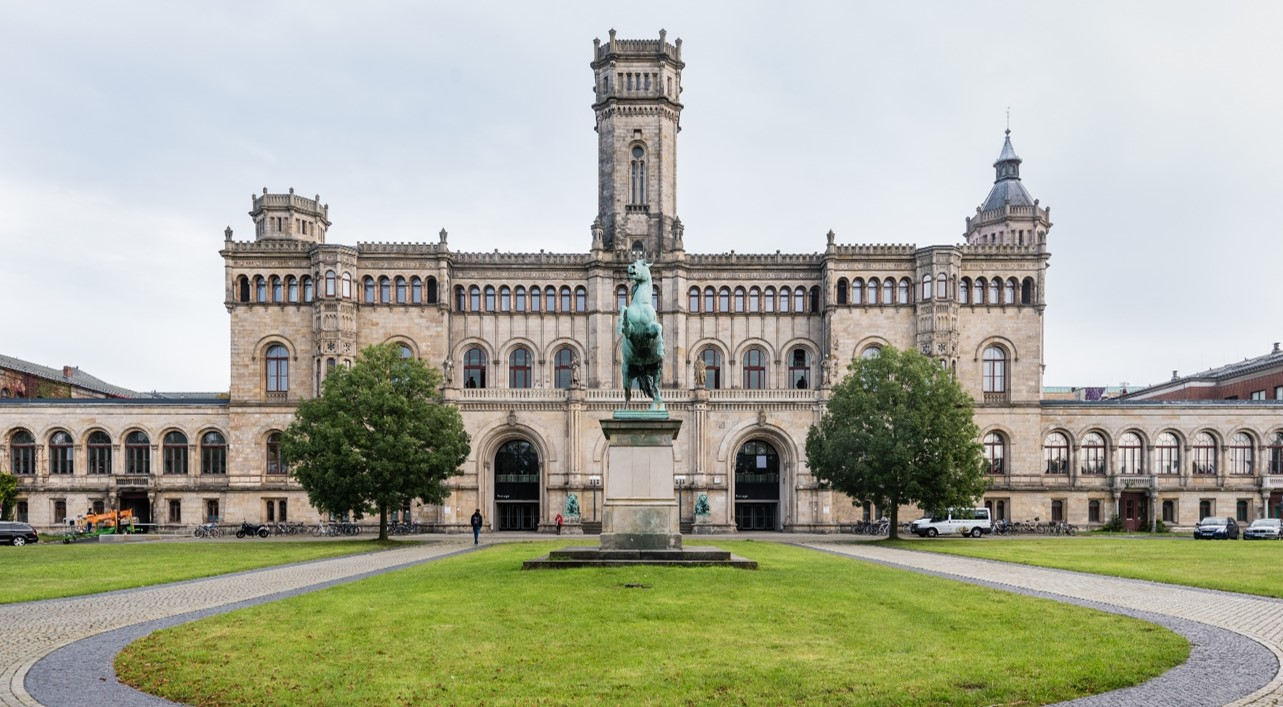
\includegraphics[width=0.75\textwidth]{figures/luh_default_presentation_title_image.jpg}}

\author[Lindauer \& Anand]{Marius Lindauer and Avishek Anand\\[1em]
	
\includegraphics[height=\logoheight]{../latex_main/figures/luh_logo_rgb_0_80_155.pdf}\qquad

\includegraphics[height=\logoheight]{../latex_main/figures/TNT_darkv4}\qquad

\includegraphics[height=\logoheight]{../latex_main/figures/L3S.jpg}	}
\date{Winter Term 2021
}


%%% Custom Packages
%----------------------------------------------------------------------
% Create dummy content
\usepackage{blindtext}

% Adds a frame with the current page layout. Just call \layout inside of a frame.
\usepackage{layout}


\title[Introduction]{iML: Feature Effects}
\subtitle{ICE and PDP}

%\institute{}


\begin{document}
	
	\maketitle

	%-----------------------------------------------------------------------------------------------------------------------------
	
\begin{frame}{Feature Effects}

\vspace{-1em}
\textbf{Feature Effects} visualize or quantify the (average) relationship between the features and the model predictions.

\begin{itemize}
    \item Methods: PD Plots, ICE curves, ALE plots
    \item Similar to regression coefficients (LMs) or Splines (GAMs).
\end{itemize}

\centerline{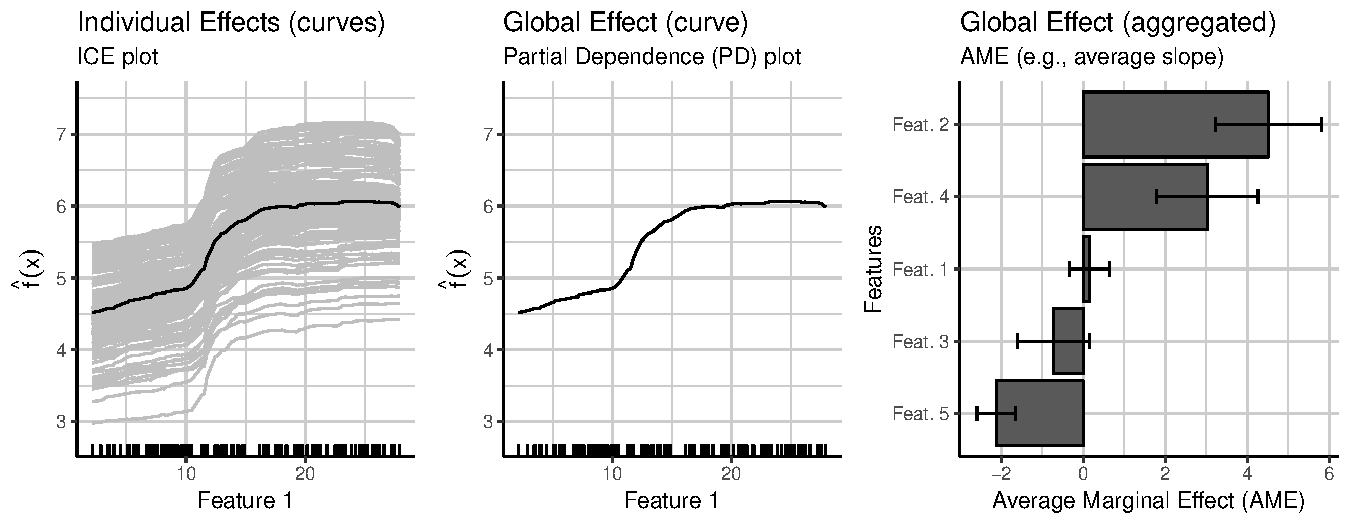
\includegraphics[width=0.7\textwidth]{figure/feature-effects.pdf}}

\begin{center}
    Individual (curves) $\xrightarrow[]{\text{aggregate}}$ Global (curve)  $\xrightarrow[]{\text{aggregate}}$ Global (number)
\end{center}

\end{frame}

\begin{frame}{Individual Conditional Expectation (ICE) \lit{Goldstein et al. 2014}{https://arxiv.org/abs/1309.6392}}

\begin{itemize}
    \item each observation $x^{(i)}$ can be partitioned into $x^{(i)}_S$ and $x^{(i)}_C$
    \begin{itemize}
        \item $x^{(i)}_S$ containing the features of interest
        \item $x^{(i)}_C$ the remaining features
    \end{itemize}
\end{itemize}  

\pause

ICE curves visualize how the model prediction of individual observations $x^{(i)}$
change by varying the feature values in $x_S$ while keeping all other features in $x^{(i)}_C$ fixed:
$$\hat{f}_{S}^{(i)}(x_S) = \hat{f}(x_S, x^{(i)}_C)$$

\pause
In practice, $x_S$ consists of one or two features.

\bigskip
\pause

\alert{Note}: $\hat{f}$ indicates we do this on our predictive model by simply querying it at different $x_S$.

\end{frame}

\begin{frame}[c]{ICE Curves}

\vspace{-0.2cm}
\begin{center}
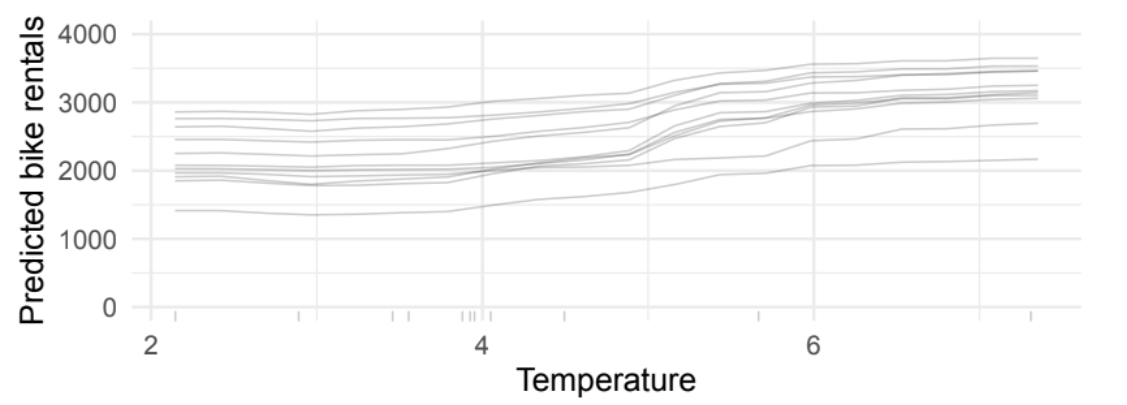
\includegraphics[width=0.7\textwidth]{figure/ICE01.png}
\end{center}
\vspace{-0.3cm}


\begin{itemize}
    \item Each line displays the change in prediction for a single observation due to varying the feature temperature.
\end{itemize}

\end{frame}

\begin{frame}[c]{Creation of ICE \lit{Scholbeck et al. 2019}{https://arxiv.org/abs/1904.03959}}

Steps to create an ICE curve of an observation regarding a single feature $x_S$ according to the \textbf{SIPA} framework:

\begin{enumerate}
\item \textbf{Sampling:} Choose grid points along $x_S$.
\item For each grid point:
\begin{itemize}
\item \textbf{Intervention:} Replace the original feature value $x_S$ with the current grid value.
\item \textbf{Prediction:} Get the model prediction with replaced feature value $x_S$.
\end{itemize}
%\item \textbf{Aggregation:} none.
\item \textbf{Visualization:} Draw a curve per observation with the grid points on the x-axis and the prediction on the y-axis.
\end{enumerate}

\end{frame}

\begin{frame}{Individual Conditional Expectation (ICE)}
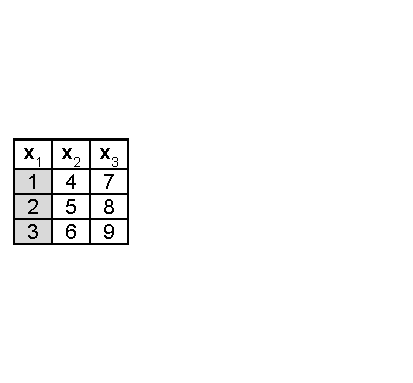
\includegraphics[page=1, width=0.35\textwidth]{figure/ice_pd_plot_demo}

\textbf{Sampling:} Choose grid points along $x_1  $ that will be used to intervene the data (here: all unique values $1, 2$ and $3$).

\end{frame}
%--------------------------------------------------------
\begin{frame}{Individual Conditional Expectation (ICE)}

\includegraphics[page=2, width=0.35\textwidth]{figure/ice_pd_plot_demo}

\textbf{Intervention:} Replace all observed values in $x_1$ for each observation with the previously sampled grid points.

\end{frame}
%--------------------------------------------------------
\begin{frame}{Individual Conditional Expectation (ICE)}

\includegraphics[page=3, width=0.35\textwidth]{figure/ice_pd_plot_demo}

\textbf{Prediction:} Make predictions and plot $\hat{f}_{1}^{(i)}(x_1)$ vs. $x_1$, where $$\hat{f}_{1}^{(i)}(x_1) = \hat{f}(x_1, x^{(i)}_{2, 3}).$$

\end{frame}
%--------------------------------------------------------
\begin{frame}{Individual Conditional Expectation (ICE)}

\begin{columns}[T]
\begin{column}{0.55\textwidth}
\vspace*{-\topsep}
\vspace*{0.5\lineskip}
\includegraphics[page=5, trim=-3.69cm 0cm 3.69cm 0cm, width=0.7\textwidth]{figure/ice_pd_plot_demo}
\end{column}
\begin{column}{0.45\textwidth}

\begin{center}
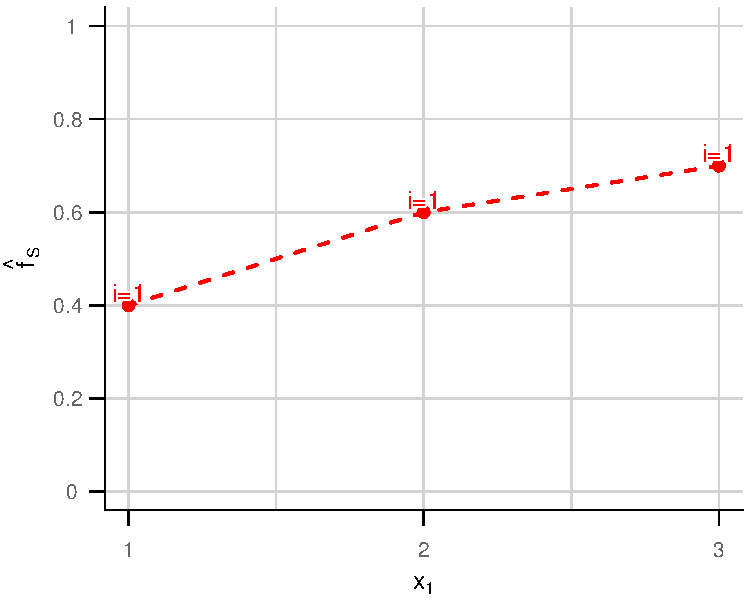
\includegraphics[page=1, width=0.9\textwidth]{figure/ICE}
\end{center}

\end{column}
\end{columns}
\vspace*{\topsep}

\textbf{Visualization:} ICE curve for observation $i=1$ connects all predictions at the corresponding grid points associated to the $i$-th observation.

\end{frame}
%--------------------------------------------------------
\begin{frame}{Individual Conditional Expectation (ICE)}


\begin{columns}[T]
\begin{column}{0.55\textwidth}
\vspace*{-\topsep}
\vspace*{0.5\lineskip}
\includegraphics[page=6, trim=-3.69cm 0cm 3.69cm 0cm, width=0.7\textwidth]{figure/ice_pd_plot_demo}
\end{column}
\begin{column}{0.45\textwidth}

\begin{center}
\includegraphics[page=2, width=0.9\textwidth]{figure/ICE}
\end{center}

\end{column}
\end{columns}
\vspace*{\topsep}

\textbf{Visualization:} ICE curve for observation $i=2$ connects all predictions at the corresponding grid points associated to the $i$-th observation.

\end{frame}
%--------------------------------------------------------
\begin{frame}{Individual Conditional Expectation (ICE)}

\begin{columns}[T]
\begin{column}{0.55\textwidth}
\vspace*{-\topsep}
\vspace*{0.5\lineskip}
\includegraphics[page=7, trim=-3.69cm 0cm 3.69cm 0cm, width=0.7\textwidth]{figure/ice_pd_plot_demo}
\end{column}
\begin{column}{0.45\textwidth}

\begin{center}
\includegraphics[page=3, width=0.9\textwidth]{figure/ICE}
\end{center}

\end{column}
\end{columns}
\vspace*{\topsep}

\textbf{Visualization:} ICE curve for observation $i=3$ connects all predictions at the corresponding grid points associated to the $i$-th observation.
\end{frame}

\begin{frame}{Partial Dependence \lit{Friedman 2001}{https://statweb.stanford.edu/~jhf/ftp/trebst.pdf} \lit{Scholbeck et al. 2019}{https://arxiv.org/abs/1904.03959}}

The partial dependence (PD) plot is the expectation of the ICE curves w.r.t. the marginal distribution of complementary features $x_C$:
$$\mathbb{E}_{x_C} \left( \hat{f}(x_S, x_C) \right) = \int_{-\infty}^{\infty} \hat{f}(x_S, x_C) \, dP(x_C)$$

For a single $x_S$, it is estimated by the point-wise average of the ICE curves:
$$\text{PD}_S := \hat{f}_{S}(x_S) = \frac{1}{n} \sum_{i=1}^n \hat{f}(x_S, x_C^{(i)})$$

%Within the SIPA framework, the partial dependence builds the \textbf{Aggregation} step.

\end{frame}


\begin{frame}{Partial Dependence: Example}
\vspace{-3em}
\begin{columns}[T]

\begin{column}{0.3\textwidth}

\begin{center}
\includegraphics[page=8, width=1\textwidth]{figure/ice_pd_plot_demo}    
\end{center}

\end{column}

\begin{column}{0.7\textwidth}

\begin{center}
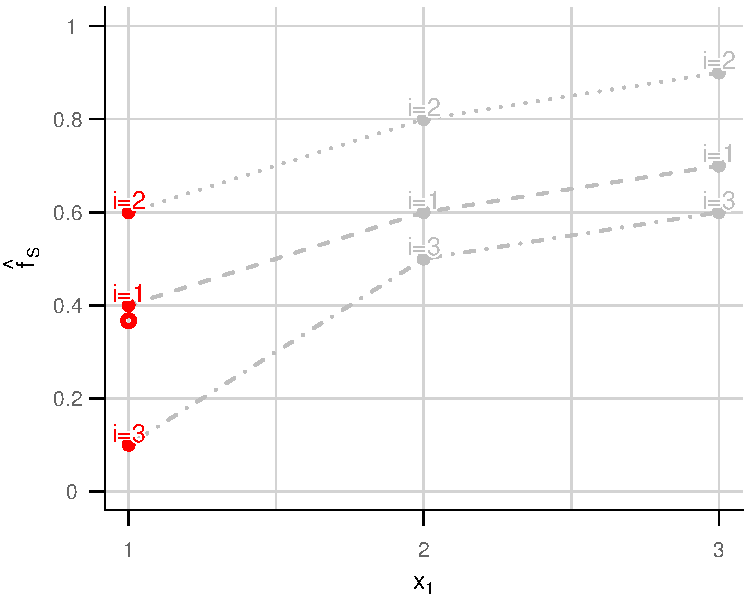
\includegraphics[page=1, width=0.6\textwidth]{figure/PD}
\end{center}

\end{column}

\end{columns}

\textbf{Aggregation:} Estimate partial dependence by the point-wise average of the ICE curves at \fcolorbox{red}{white}{$x_S = x_1 = 1$}:
$$PD_1 = \hat{f}_{1}(x_1) = \frac{1}{n} \sum_{i=1}^n \hat{f}(x_1, x_{2, 3}^{(i)})$$

\end{frame}


\begin{frame}{Partial Dependence: Example}
\vspace{-3em}
\begin{columns}[T]

\begin{column}{0.3\textwidth}

\begin{center}
\includegraphics[page=9, width=1\textwidth]{figure/ice_pd_plot_demo}
\end{center}
\end{column}


\begin{column}{0.7\textwidth}

\begin{center}
\includegraphics[page=2, width=0.6\textwidth]{figure/PD}
\end{center}

\end{column}

\end{columns}

\textbf{Aggregation:} Estimate partial dependence by the point-wise average of the ICE curves at \fcolorbox{red}{white}{$x_S = x_1 = 2$}:
$$PD_1 = \hat{f}_{1}(x_1) = \frac{1}{n} \sum_{i=1}^n \hat{f}(x_1, x_{2, 3}^{(i)})$$

\end{frame}


\begin{frame}{Partial Dependence: Example}
\vspace{-3em}
\begin{columns}[T]

\begin{column}{0.3\textwidth}

\begin{center}
\includegraphics[page=10, width=\textwidth]{figure/ice_pd_plot_demo}
\end{center}

\end{column}
\begin{column}{0.7\textwidth}

\begin{center}
\includegraphics[page=3, width=0.6\textwidth]{figure/PD}
\end{center}
\end{column}

\end{columns}

\textbf{Aggregation:} Estimate partial dependence by the point-wise average of the ICE curves at \fcolorbox{red}{white}{$x_S = x_1 = 3$}:
$$PD_1 = \hat{f}_{1}(x_1) = \frac{1}{n} \sum_{i=1}^n \hat{f}(x_1, x_{2, 3}^{(i)})$$

\end{frame}

\begin{frame}{Partial Dependence: Example}
\vspace{-3em}
\begin{columns}[T]

\begin{column}{0.3\textwidth}

\begin{center}
\includegraphics[page=10, width=\textwidth]{figure/ice_pd_plot_demo}
\end{center}

\end{column}
\begin{column}{0.7\textwidth}

\begin{center}
\includegraphics[page=3, width=0.6\textwidth]{figure/PD}
\end{center}
\end{column}

\end{columns}

\textbf{Aggregation:} Estimate partial dependence by the point-wise average of the ICE curves at \fcolorbox{red}{white}{$x_S = x_1 = 3$}:
$$PD_1 = \hat{f}_{1}(x_1) = \frac{1}{n} \sum_{i=1}^n \hat{f}(x_1, x_{2, 3}^{(i)})$$

\end{frame}

\begin{frame}[c]{Further Material}

\begin{itemize}
    \item Blog "Efficient Partial Dependence Plots with decision trees" by \lit{Nicolas Hug 2019}{http://nicolas-hug.com/blog/pdps}
\end{itemize}

\end{frame}

\end{document}
